\documentclass[10pt, aspectratio=169]{beamer}

% handout
% \documentclass[handout, 10pt]{beamer}

\usepackage{clases}

\title{Investigación Operativa}
\subtitle{Programaci\'on Lineal Entera - Branch \& Bound}
\date{}
\author{Facundo Gutiérrez - Nazareno Faillace Mullen}
\institute{Departamento de Matemática - FCEN - UBA}
% \titlegraphic{\hfill\includegraphics[height=1.5cm]{logo.pdf}}

\begin{document}

\maketitle

\begin{frame}{Problema Lineal Entero}
    
    \begin{itemize}
        \item Programación Lineal:
        \begin{itemize}
            \normalsize
            \item Simplex $\rightarrow$ complejidad exponencial (pero \textit{usualmente es polinomial} \footnote{Spielman \& Teng, \textit{Smoothed Analysis of Algorithms: Why the Simplex Algorithm Usually Takes Polynomial Time}, 2001, \color{blue}\url{https://arxiv.org/abs/cs/0111050}})
            \item Método de elipsoides $\rightarrow$ complejidad polinomial
            \item Método de punto interior $\rightarrow$ complejidad polinomial
        \end{itemize}
        $\Rightarrow$ resolver Problemas Lineales es ``fácil".
        \vspace{1cm}
        \item Programación Lineal Entera:
        \begin{itemize}
            \normalsize
            \item NP-Completo $\Rightarrow$ resolver problemas de Programación Lineal Entera es difícil.
        \end{itemize}
    \end{itemize}

    \textbf{Idea:} resolver Programación Lineal Entera usando Programación Lineal.
\end{frame}

\begin{frame}{Problema Lineal Entero}
	El objetivo de la clase de hoy ser\'a resolver el problema:
	
	$$
	\begin{matrix}
	& \hspace{1cm} & \max & c^t x       \\ 
	& \hspace{1cm} & \text{s.a:}  & Ax \leq b \\      
    & \hspace{1cm} &	         &  x \in \color{goodgreen}{\mathbb{Z}}_{\geq 0}^n  \\
	\end{matrix}
	$$
	
	% Veamos primero c\'omo se relaciona este problema con la c\'apsula convexa de los puntos factibles, antes de adentrarnos a resolver el problema en s\'i.
\end{frame}

\begin{frame}{}
    \[
        \begin{array}{rl}
            \max & c^t x \\
             \text{s.a:}& Ax \leq b \\
              & x \in \mathbb{Z}^n_{\geq 0}
        \end{array}
    \]
    Llamamos $\mathcal{S}=\{x \in \mathbb{Z}^n_{\geq 0}\colon Ax \leq b\}$ la región de soluciones factibles.
    
    Dos ideas para entender Branch \& Bound:
    \begin{enumerate}
        \item Para todo $\mathcal{T}$ tal que $\mathcal{S}\subseteq \mathcal{T}$ vale:  $\zopt_{\mathcal{S}} \leq \zopt_{\mathcal{T}}$ 
        \item $\zopt_{\mathcal{S}}= \zopt_{conv(\mathcal{S})}$
    \end{enumerate}

    \textbf{Obs:} \textbf{hallar $\zopt_{conv(\mathcal{S})}$ es un problema de Programación Lineal }
\end{frame}

\begin{frame}{}

    \textit{Idea de la demo del punto 2:}
    
	Llamemos $\mathcal{S} = \left \{ Ax \leq b, x \in \mathbb{Z}_{\geq 0}^n \right \}$. Supongamos por simplicidad que $\mathcal{S} \neq \varnothing$ y que adem\'as es acotado (y por ende tiene solo finitos puntos). Nosotros buscamos el valor de $z_{\text{IP}} = \max \left \{ c^tx : x \in \mathcal{S} \right \}$.
	
	 Como son solo finitos puntos, adem\'as de realizarse en alg\'un punto que llamaremos $x^*$, tenemos que $c^tx^* = z_{\text{IP}} < \infty$ 
	\pause
	
	 Dada una combinaci\'on convexa de puntos de $\mathcal{S}$, el valor de la funci\'on objetivo est\'a acotado por $z_{\text{IP}}$, pues si $\sum\limits_{i = 1}^k \lambda_i = 1$ (con $\lambda_i \geq 0 \quad \forall i$), entonces $c^t \left ( \sum\limits_{i = 1}^k \lambda_ix_i \right ) = \sum\limits_{i = 1}^k \lambda_i\left ( c^tx_i \right ) \leq \sum\limits_{i = 1}^k \lambda_iz_{\text{IP}} = z_{\text{IP}} = c^tx^*$.
	 \pause
	 
	 Concluimos que $z_{\text{IP}} = \max \left \{ c^tx : x \in \mathcal{S} \right \} = \max \left \{ c^tx : x \in \text{conv}(\mathcal{S}) \right \}$, pues $x^* \in \mathcal{S} \subseteq \text{conv}(\mathcal{S})$. La diferencia est\'a en que este \'ultimo es un problema lineal (y la dificultad radica en describir $\text{conv}(\mathcal{S})$, la c\'apsula convexa de  $\mathcal{S}$)
\end{frame}

\begin{frame}{C\'apsula convexa - Ejemplo 2D}
\begin{minipage}{0.45\textwidth}
	$$
	\begin{matrix}
	 \text{m\'ax} & y      & &   \\ 
 	 \text{s.a:}  & -x +y  & \leq &  1 \\      
 	 			  & 3x +2y & \leq & 12 \\
   	 			  & 2x +3y & \leq & 12 \\
                  &  x,y \in \color{goodgreen}{\mathbb{Z}}_{\geq 0}  \\
	\end{matrix}
	$$
\end{minipage}
\begin{minipage}{0.45\textwidth}
	$$
	\begin{matrix}
	 \text{m\'ax} & y      & &   \\ 
 	 \text{s.a:}  & -x +y  & \leq &  1 \\      
 	 			  & 3x +2y & \leq & 12 \\
   	 			  & 2x +3y & \leq & 12 \\
                  &  x,y \in \color{blue}{\mathbb{R}}_{\geq 0}  \\
	\end{matrix}
	$$
\end{minipage}
\pause
\begin{center}
	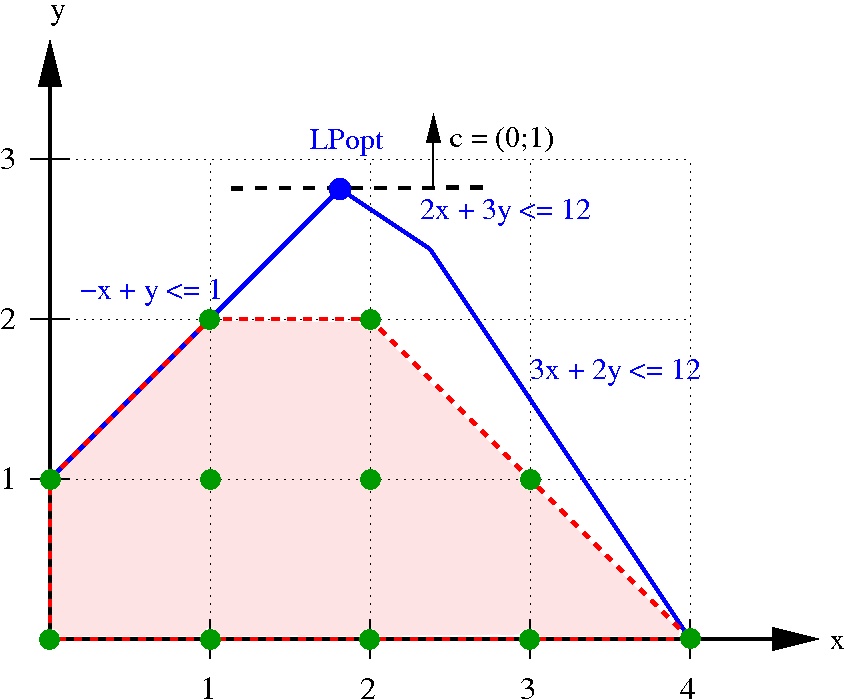
\includegraphics[scale=0.2]{imagenes/chull2d.png}
\end{center}


\end{frame}

\begin{frame}{C\'apsula convexa - Ejemplo 3D (gr\'afico) }

\begin{center}
	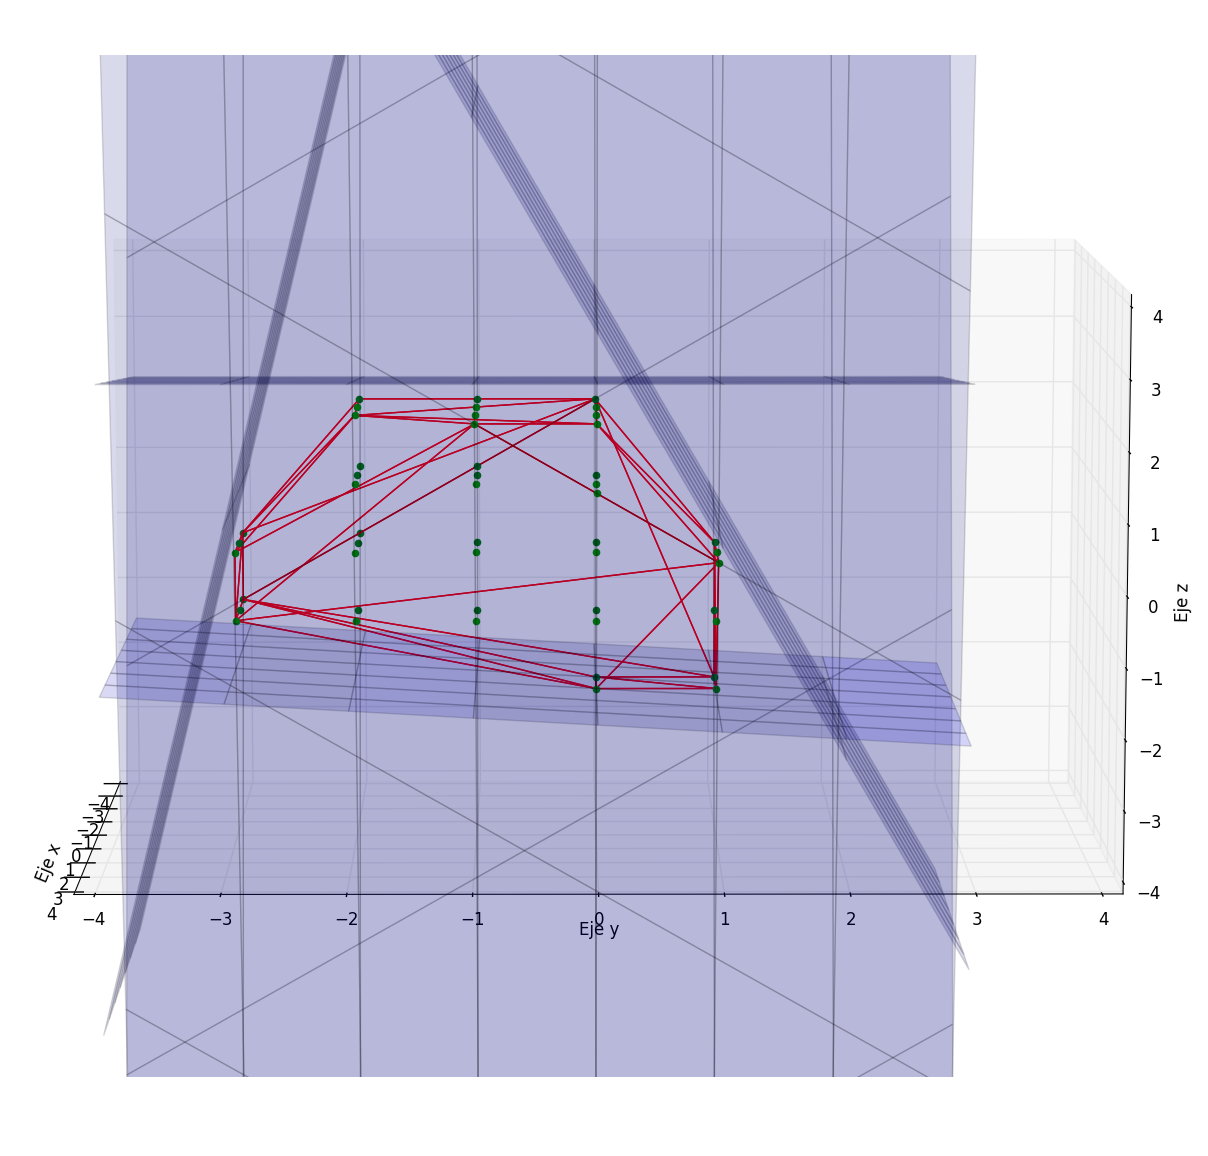
\includegraphics[scale=0.3]{imagenes/chull3d.png}	
\end{center}

\end{frame}

\begin{frame}{Relajaci\'on lineal de un problema entero}
	Dado un problema de PLE (Programaci\'on Lineal Entera) de la forma:
	
	$$
	\begin{matrix}
	& \hspace{1cm} & \max & c^t x       \\ 
 \Large{\text{(IP)}}	& \hspace{1cm} & \text{s.a:}  & Ax \leq b \\      
    & \hspace{1cm} &	         &  x \in \color{goodgreen}{\mathbb{Z}}_{\geq 0}^n  \\
	\end{matrix}
	$$
  	\pause
	Definimos su \textsl{relajaci\'on lineal} al problema que se obtiene al relajar la condici\'on de integralidad de las variables en cuesti\'on:
	
	$$
	\begin{matrix}
	& \hspace{1cm} & \max & c^t x       \\ 
 \Large{\text{(LP)}}	& \hspace{1cm} & \text{s.a:}  & Ax \leq b \\      
    & \hspace{1cm} &	         &  x \in \color{blue}{\mathbb{R}}_{\geq 0}^n  \\
	\end{matrix}
	$$
	\pause
	
	\textbf{Observaci\'on}: Usando lo visto en las clases anteriores, tenemos las herramientas para encontrar el \'optimo de la relajaci\'on lineal. 
    
\end{frame}


\begin{frame}{Redondear soluciones de la relajaci\'on lineal}
No siempre redondear la soluci\'on de la relajaci\'on lineal es adecuado:

\begin{minipage}{0.48\textwidth}

	\begin{center}
			\textbf{Podr\'ia no ser \'optima}
		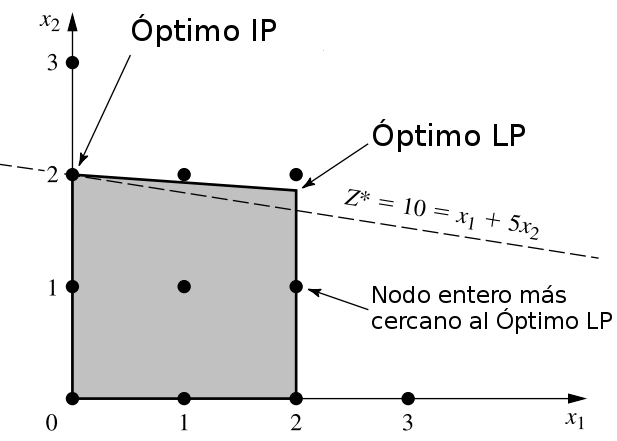
\includegraphics[width=\textwidth]{imagenes/redondeo_relajacion_suboptimo.png}
	\end{center}
\end{minipage}
\begin{minipage}{0.48\textwidth}

	\begin{center}
		\textbf{Podr\'ia no ser factible}
		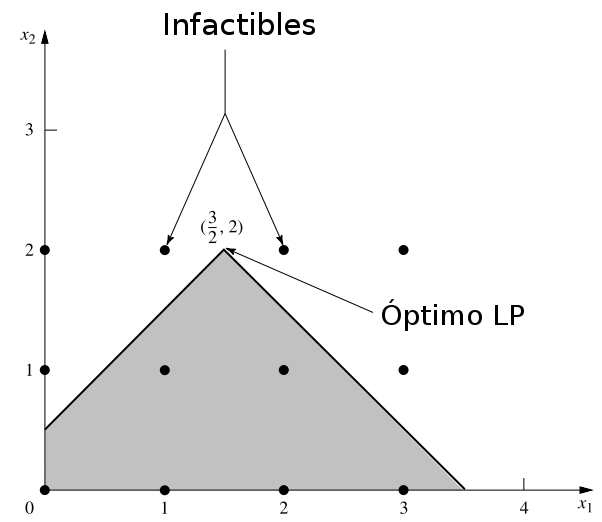
\includegraphics[width=\textwidth]{imagenes/redondeo_relajacion_infactible.png}
	\end{center}
\end{minipage}

\end{frame}

% \begin{frame}{Idea}
%     Sean dos problemas de optimización:
%     \begin{columns}
%         \column{0.5\textwidth}
%         \[
%         \begin{array}{lrl}
%             (A) & \max & c^tx \\
%             & \text{s.a:} & x\in S 
%         \end{array}
%         \]
%         \column{0.5\textwidth}
%         \[
%         \begin{array}{lrl}
%             (B) & \max & c^tx \\
%              & \text{s.a:} & x\in T 
%         \end{array}
%         \]
%     \end{columns}
%     tales que $S\subset T$. Sean $z^\ast$ el valor de la función objetivo en el óptimo de (A) y $\hat{z}^\ast$ el valor de la función objetivo en el óptimo de (B), entonces $\zopt \leq \hat{z}^\ast$
% \end{frame}


\begin{frame}{Branch \& Bound}

	La idea central del algoritmo, y que ser\'a uno de los criterios de corte a tener en cuenta, radica en la siguiente observaci\'on. 
	\pause
	
	\textsl{\textbf{Si la soluci\'on de la relajaci\'on lineal de un problema tiene todas sus coordenadas enteras, entonces tambi\'en es soluci\'on al problema entero}}
	\pause
	
	Recordemos que estamos maximizando. Si el \'optimo de la relajaci\'on (que tiene coordenadas enteras) ocurre en $x$, tenemos que: 
	$$z_{\text{IP}} \underset{(1)}{\leq} z_{\text{LP}} = c^tx \underset{(2)}{\leq} z_{\text{IP}} \Rightarrow z_{\text{IP}} = z_{\text{LP}}	$$

    \pause

    \begin{enumerate}
        \item[(1)] pues $\{x \in \mathbb{Z}^n_{\geq 0}\colon Ax \leq b\} \subseteq \{x \in \mathbb{R}^n_{\geq 0}\colon Ax \leq b\}$
        \item[(2)] como $x$ tiene todas sus coordenadas enteras:  $x\in \{x \in \mathbb{Z}^n_{\geq 0}\colon Ax \leq b\}$
    \end{enumerate}
 
	\pause
	Normalmente la soluci\'on de la relajaci\'on lineal de nuestro problema no tiene por qu\'e dar un punto con todas sus coordenadas enteras. 
	Si esto ocurre, vamos a particionar el espacio de b\'usqueda en otros m\'as pequeños donde buscamos soluciones de la misma forma (¡sin dejar de lado v\'ertices enteros al particionar!).
	
\end{frame}

\begin{frame}{Branch \& Bound - Criterios de Poda}

	Observemos qu\'e informaci\'on podemos deducir de un problema entero en funci\'on del resultado obtenido al resolver su relajaci\'on lineal.
	\pause
	\begin{enumerate}
		\item Si la \textsl{relajaci\'on lineal} es \textbf{infactible}, entonces nuestro problema en cuesti\'on tambi\'en es infactible. 
		\pause
		\item Si la \textsl{relajaci\'on lineal} tiene un \textbf{\'optimo con todas sus coordenadas enteras}, entonces el problema entero en cuesti\'on est\'a resuelto y el \'optimo coincide.  
		\pause
		\item \textbf{Toda soluci\'on entera} tendr\'a un \textbf{valor menor} al de la  \textsl{relajaci\'on lineal}.  
	\end{enumerate}
	
\end{frame}

\begin{frame}{Branch \& Bound - Criterios de Poda}

	A lo largo del algoritmo vamos a mantener una colecci\'on de problemas enteros a resolver, y el valor de la mejor soluci\'on entera obtenida hasta el momento (\textsl{\textbf{valor incumbente}}). 
	\pause
	
	Esto nos da otra observaci\'on a tener en cuenta durante el algoritmo.
	\begin{enumerate}
		\item[4.] Si el valor \textbf{\'optimo} de la \textsl{relajaci\'on lineal} es \textbf{menor al \textsl{valor incumbente}}, entonces no hace falta terminar de resolver el problema entero en cuesti\'on.
	\end{enumerate}
\end{frame}

\begin{frame}{Branch \& Bound - Algoritmo}
Juntando todas estas ideas, podemos formular un algoritmo para resolver un problema lineal entero, para el cual introducimos la siguiente notaci\'on.
\pause
\begin{itemize}
	\item $z_{\text{IP}}^i$ al \textsl{valor incumbente} de la mejor soluci\'on encontrada 
	\item $\mathcal{L}$ a la lista de problemas que quedan por resolver
	\item $\mathcal{S}^i$ ser\'a la $i$-\'esima regi\'on a considerar y $\bar{z}_{\text{R}}^i$ su \textsl{cota incumbente}
\end{itemize}
\pause
\begin{enumerate}
	\item $\mathcal{L} = \{\mathcal{S}\}, z_{\text{IP}}^0 = -\infty$
	
\item Mientras $\mathcal{L}$ no est\'e vac\'io: (Si $\mathcal{L} = \varnothing$ terminamos)

\begin{enumerate}
		\item {\color<4->{red} Sacar alg\'un $\mathcal{S}^i \in \mathcal{L}$}. Resolver su relajaci\'on con \'optimo $z_R^i$ en $x_R^i$ (si la relajaci\'on es infactible no hace falta hacer nada).
		\item Si $z_R^i > z_{\text{IP}}^i$ y $x_R^i$ entera: Actualizar la soluci\'on y el \textsl{valor incumbente}. Sacar de $\mathcal{L}$ todos los problemas $\mathcal{S}^j$ con $\bar{z}_{\text{R}}^j \leq z_{\text{R}}^i = z_{\text{IP}}^{i+1}$
		\item Si $z_R^i > z_{\text{IP}}^i$ y $x_R^i$ no es entera : {\color<4->{red} Particionar $\mathcal{S}^i$} en $\{ \mathcal{S}_j^i \}_{j = 1}^k$, y agregar a $\mathcal{S}_j^i$ a $\mathcal{L}$ con  $\bar{z_R}_j^i = z_R^i$

\end{enumerate}

\end{enumerate}

\end{frame}

\begin{frame}{Branch \& Bound - Particionar Problemas}
	Dado un problema, la forma que utilizaremos para obtener un subproblema a partir del mismo ser\'a agregando una restricci\'on.

	En el $i-$\'esimo paso, si tenemos $x_R^i \not\in \mathcal{S}^i$, entonces  tiene alguna coordenada que no es entera. Sea $j$ tal que ${x_R}_j^i \not\in \mathbb{Z}$, particionamos $\mathcal{S}^i$ en dos subproblemas $\mathcal{S}_1^i$ y $ \mathcal{S}_2^i$ agregando las restricciones $x_j \leq \left \lfloor {x_R}_j^i \right \rfloor$ en $\mathcal{S}_1^i$ y $x_j \geq \left \lceil {x_R}_j^i \right \rceil$ en $\mathcal{S}_2^i$.
	\pause
	
	% Dependiendo de nuestro problema, podemos optar por distintas formas de particionar. La que vimos anteriormente funciona en cualquier caso y se la conoce como \textsl{``variable dichotomy"}. En caso de haber varios $j$ tal que ${x_R}_j^i \not\in \mathbb{Z}$, conviene fijar alg\'un criterio (que idealmente depender\'a de nuestro problema)
	
\end{frame}

\begin{frame}{Branch \& Bound - Elecci\'on del pr\'oximo problema}
    % \footnotesize
	% Las formas de elegir el pr\'oximo subproblema a tratar se dividen en dos grupos, seg\'un si seguimos reglas definidas \textsl{a priori}, o utilizamos reglas \textsl{adaptativas} seg\'un la informaci\'on obtenida en cada subproblema (cotas incumbentes por ejemplo). 
	% \pause
	
	La m\'as utilizada 
 %del primer tipo 
 es la \textsl{b\'usqueda en profundidad}, donde el pr\'oximo problema a considerar es un subproblema del \'ultimo problema visto. En caso de terminar de considerar un problema, volvemos al \'ultimo que vimos que todav\'ia tenga subproblemas por considerar.

	\pause
\begin{center}
	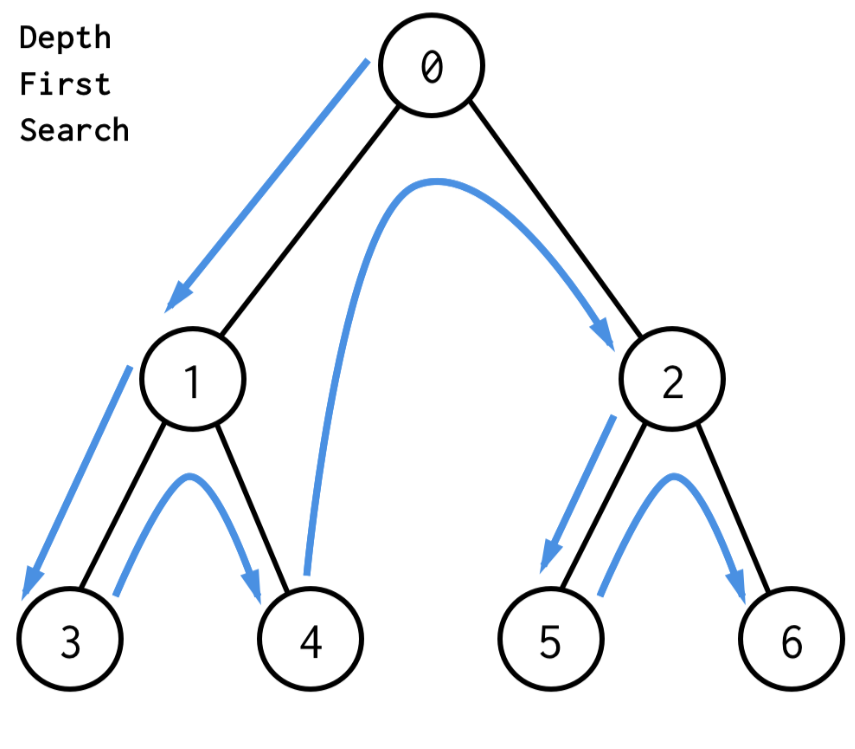
\includegraphics[scale=0.25]{imagenes/binary_DFS.png}	
\end{center}
	
\end{frame}

% \begin{frame}{Branch \& Bound - Elecci\'on del pr\'oximo problema}
	
% 	Notemos que en todo momento, tenemos una cota de cu\'an lejos estamos del \'optimo. Pues el \textsl{valor incumbente} nos da una cota inferior a nuestra soluci\'on, y al resolver una relajaci\'on lineal tenemos una cota superior al valor del \'optimo. Por lo tanto, en todo momento vale la siguiente relaci\'on:
	
% 	$$ z_{\text{IP}}^i \leq z_{\text{IP}} \leq \underset{i \in \mathcal{L}}{\max } \hspace{0.1cm} \bar{z}_R^i $$ 
	
% 	De aqu\'i, una regla adaptativa que surge naturalmente es la de resolver el subproblema que tenga mayor valor de $\bar{z}_R^i $, de forma de reducir la expresi\'on del lado derecho (o encontrar una soluci\'on factible que tenga dicho valor).

% \end{frame}

\begin{frame}{Ejemplo}
	$$
	\begin{matrix}
	 \max		 & 5x_1 + 7x_2 &          \\ 
	 \text{s.a:} & x_1 + x_2   & \leq & 6  \\      
				 & 5x_1 + 9x_2 & \leq & 45 \\
 				 & x_1,x_2 \in \mathbb{Z}_{\geq 0}&  & \\
	\end{matrix}
	$$

    Vamos a resolverlo eligiendo a $x_2$ como la primera variable a ramificar.
    
    \textbf{Ejercicio:} resolverlo eligiendo a $x_1$ como la primera variable a ramificar.
\end{frame}

% \begin{frame}{Ejemplo}
% 	$$
% 	\begin{matrix}
% 	 \max		 & 5x_1 + 7x_2 &          \\ 
% 	 \text{s.a:} & x_1 + x_2   & \leq & 6  \\      
% 				 & 5x_1 + 9x_2 & \leq & 45 \\
%  				 & x_1,x_2 \in \mathbb{Z}_{\geq 0}&  & \\
% 	\end{matrix}
% 	$$
% 	\only<1>{
% 	\begin{center}
% 		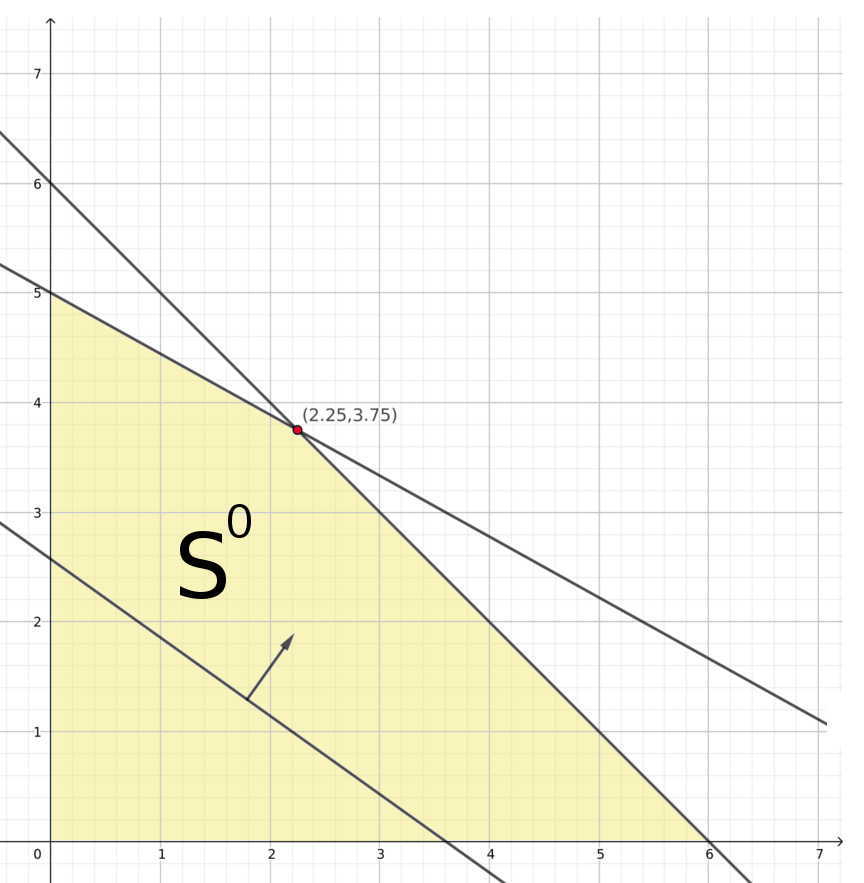
\includegraphics[scale=0.18]{imagenes/ejemplo_1_1.png}
% 	\end{center}		
% 	}
% 	\pause
% 	\only<2>
% 	{
% 	\begin{center}
% 		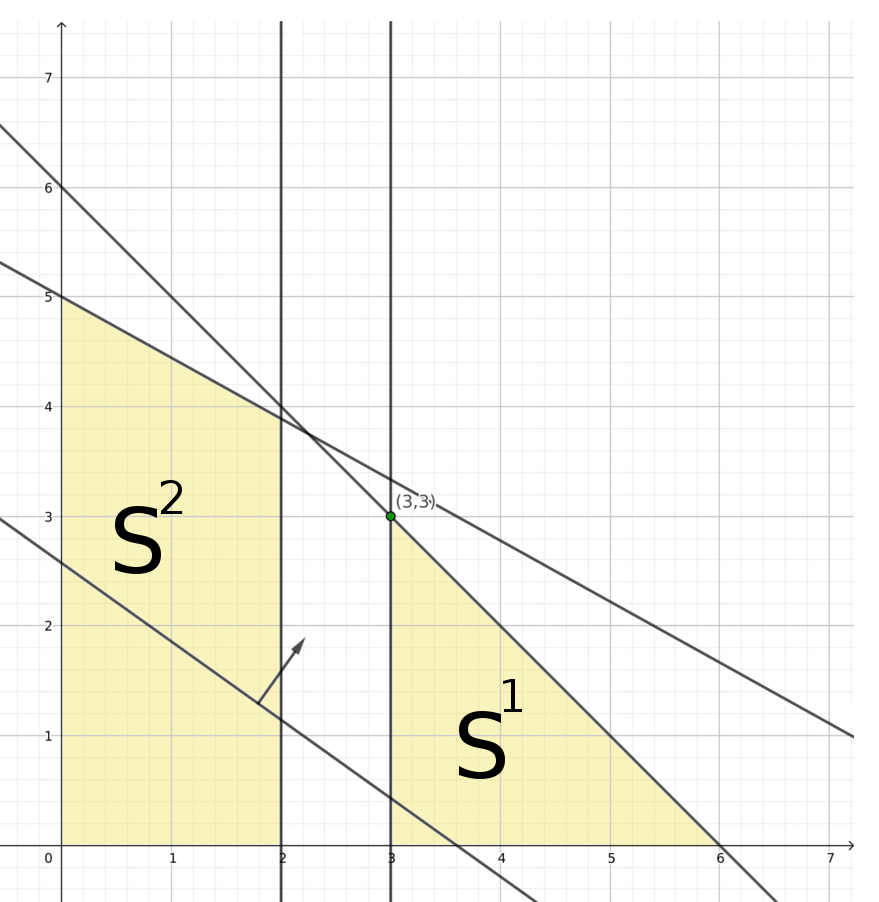
\includegraphics[scale=0.18]{imagenes/ejemplo_1_2.png}
% 	\end{center}		
% 	}
% 	\pause
% 	\only<3>
% 	{
% 	\begin{center}
% 		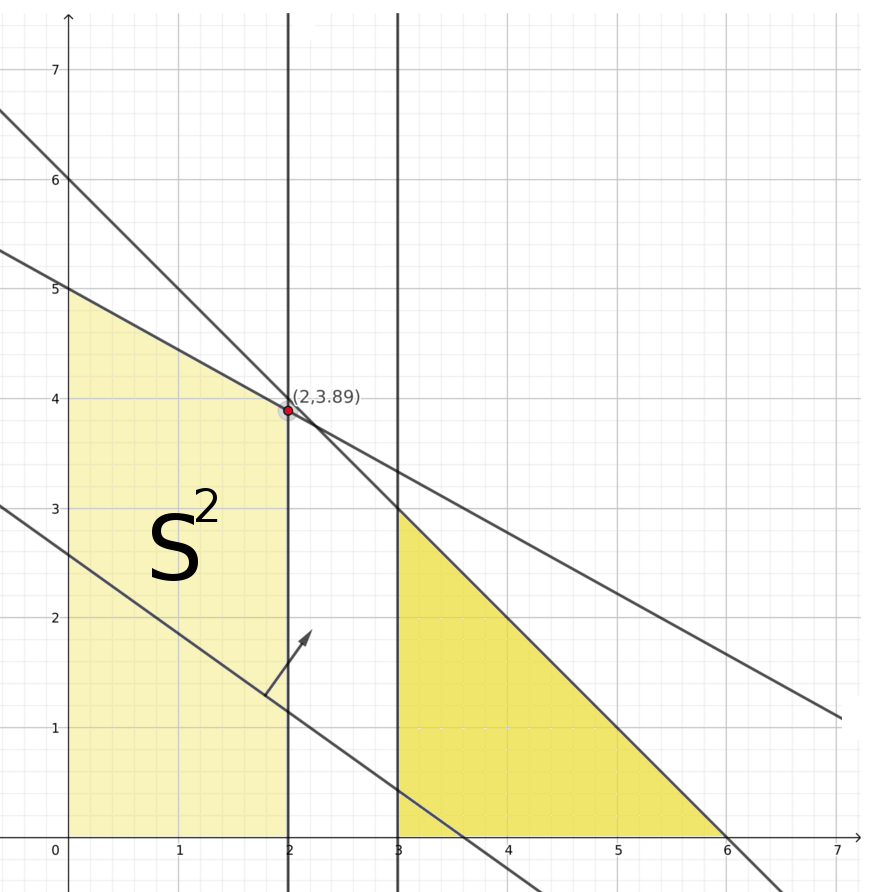
\includegraphics[scale=0.18]{imagenes/ejemplo_1_3.png}
% 	\end{center}		
% 	}
% 	\pause
% 	\only<4>{
% 	\begin{center}
% 		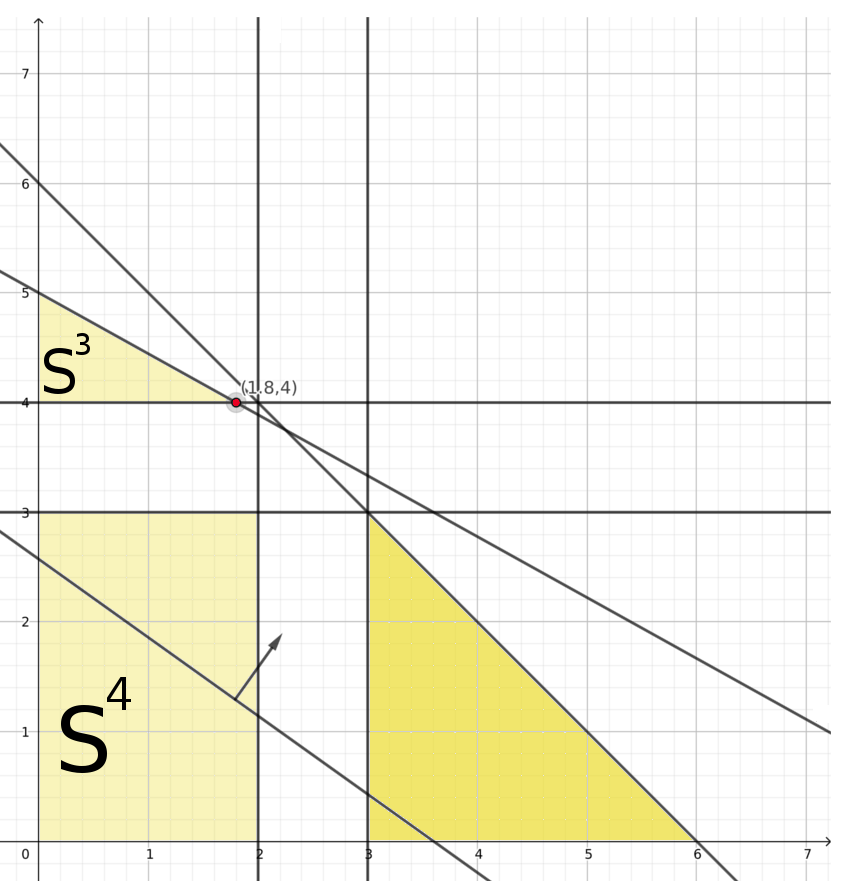
\includegraphics[scale=0.18]{imagenes/ejemplo_1_4.png}
% 	\end{center}		
% 	}
% 	\pause
% 	\only<5>
% 	{
% 	\begin{center}
% 		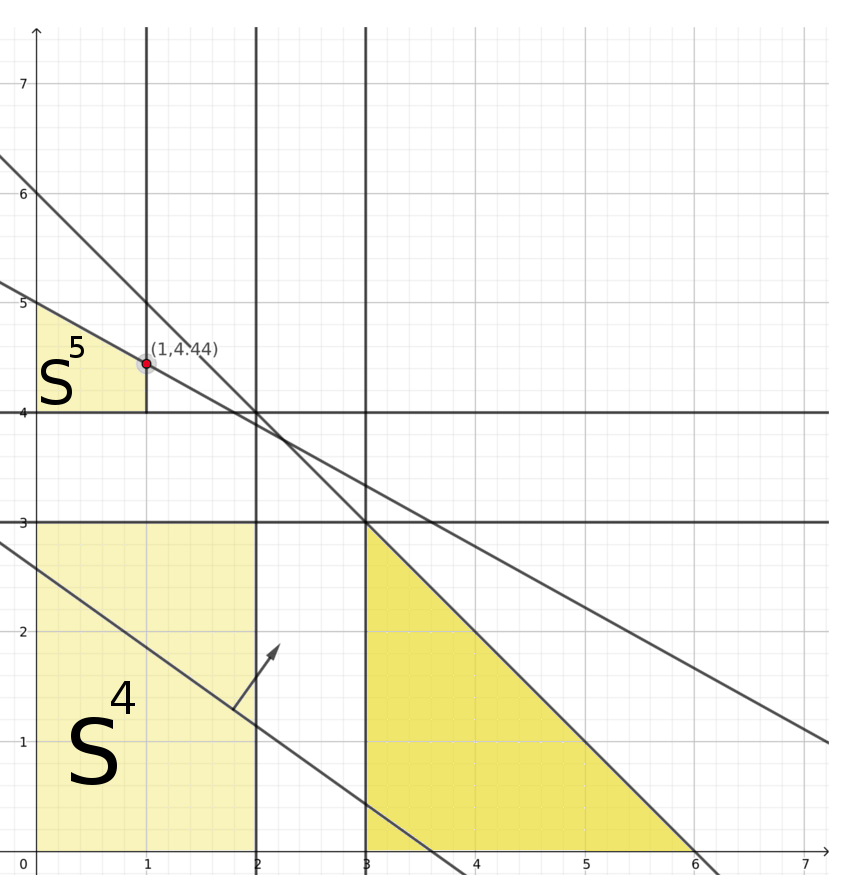
\includegraphics[scale=0.18]{imagenes/ejemplo_1_5.png}
% 	\end{center}		
% 	}
% 	\pause
% 	\only<6>
% 	{
% 	\begin{center}
% 		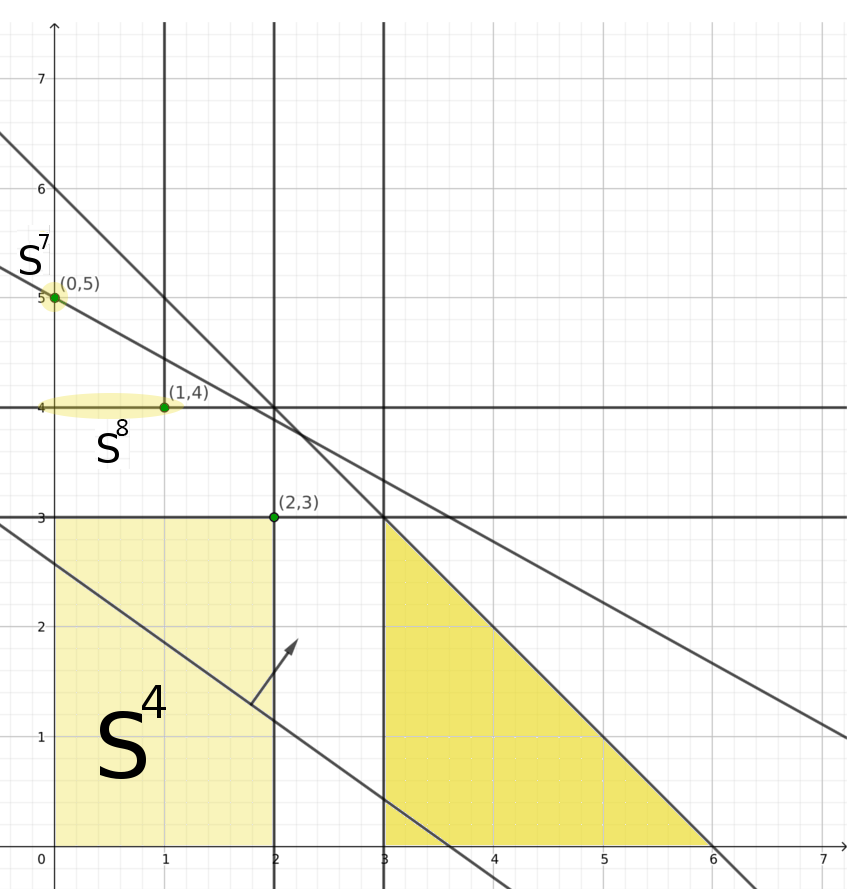
\includegraphics[scale=0.18]{imagenes/ejemplo_1_6.png}
% 	\end{center}		
% 	}
% 	\only<7>
% 	{
% 	\begin{center}
% 		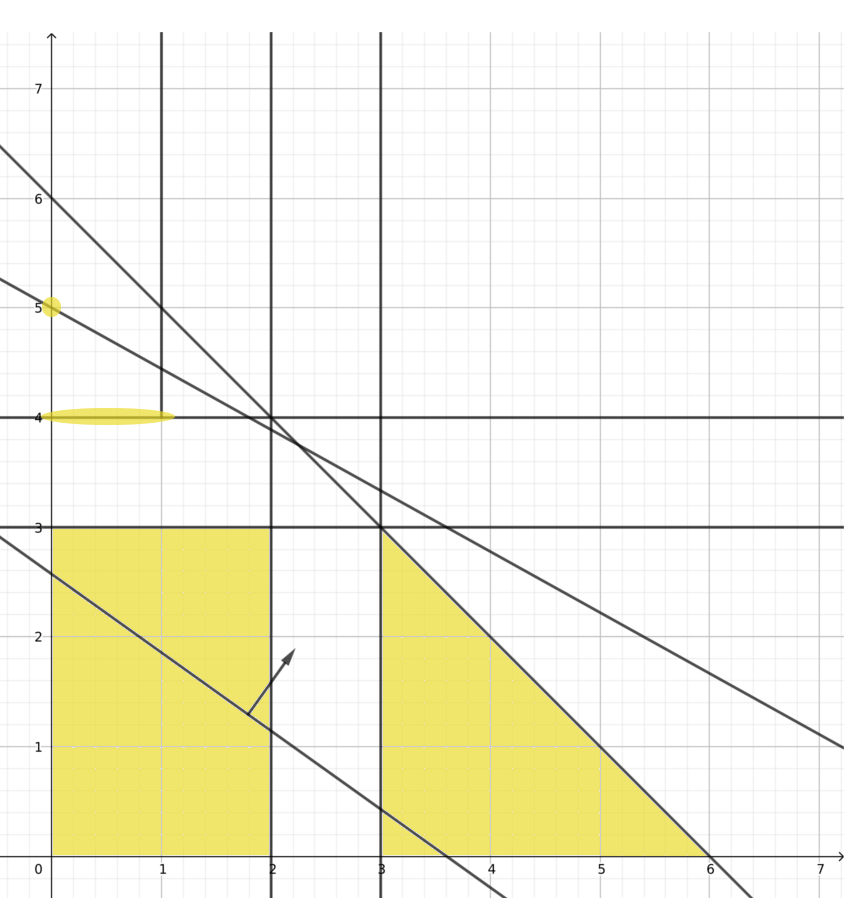
\includegraphics[scale=0.18]{imagenes/ejemplo_1_7.png}
% 	\end{center}		
% 	}
% \end{frame}

\begin{frame}{Otro ejemplo}
    \[
    \begin{array}{rrl}
        \max & 2x_1+3x_2 & \\
        \text{s.a:} & -\frac{2}{3}x_1 + x_2 & \leq \frac{5}{2} \\
        & \frac{1}{3}x_1 + x_2 & \leq \frac{9}{2} \\
        & 2x_1 + x_2 & \leq 14 \\
        & x_1, x_2\in\mathbb{Z}_{\geq 0} &
    \end{array}
    \]
\end{frame}



\begin{frame}{Branch \& Bound - Particionar Problemas}
	
	Imaginemos ahora que en el problema en cuesti\'on nuestras variables son binarias y tenemos una restricci\'on de la siguiente forma (se las conoce como GUB, de \textsl{Generalized Upper Bound constraint} y surgen naturalmente al modelar problemas):
	$$ \sum\limits_{j \in \mathcal{Q}} x_j = 1 $$
	
	Al resolver la relajaci\'on lineal, obtenemos que $0 < x_k < 1$ con $k \in \mathcal{Q}$, ¿Parece sensato separar en los problemas con $x_k = 1$ y $x_k = 0$?
	
	\pause
	
	Sin ninguna informaci\'on extra, al considerar el subproblema con $x_k = 0$ tenemos un problema muy similar al que ten\'iamos originalmente. En general conviene dividir a la regi\'on factible en subproblemas de tamaño similar, por ejemplo, podemos tomar $\mathcal{Q} = \mathcal{Q}_1 \overset{d}{\cup} \mathcal{Q}_2$ y $\# \mathcal{Q}_1 \sim \# \mathcal{Q}_2$ y separar en subproblemas que agreguen la restricci\'on 	$$ \sum\limits_{j \in \mathcal{Q}_i} x_j = 0 $$
	
\end{frame}

% \begin{frame}{Problema de la Mochila}
% 	Dados $n$ objetos, cada uno con peso $w_i > 0$, valor $v_i$ y una capacidad global $W$. Buscamos encontrar el subconjunto de objetos con mayor suma de valor que tenga suma de pesos menor o igual a $W$
% 	\pause
	
% 	$$
%  \begin{matrix}
%  \max & \sum\limits_{i = 1}^n x_iv_i &     \\ 
%  \text{s.a:}  & \sum\limits_{i = 1}^n x_iw_i & \leq W  \\      
% 	          &  x_i \in \{0,1\} & \forall i \in \{1,\dots,n\}   \\
% 	\end{matrix}
% 	$$
	
% 	\pause
% 	\textbf{Observaci\'on}: La relajaci\'on lineal al problema puede resolverse de manera sencilla.	
	
% \end{frame}

% \begin{frame}{Problema de la Mochila Fraccionario}
% 	En el caso de que podemos utilizar cantidades infinitesimalmente pequeñas de cada objeto, obtenemos el siguiente problema: 
% 	$$
%  \begin{matrix}
%  \max & \sum\limits_{i = 1}^n x_iv_i &     \\ 
%  \text{s.a:}  & \sum\limits_{i = 1}^n x_iw_i & \leq W  \\      
% 	          & 0 \leq x_i \leq 1 & \forall i \in \{1,\dots,n\}   \\
% 	\end{matrix}
% 	$$
% 	\pause
	
% 	La soluci\'on se resume al siguiente \textbf{algoritmo goloso}:
	
% 	\textsl{Siempre conviene utilizar la mayor cantidad posible del objeto que tenga mayor valor por unidad de peso}
	
% 	Es decir, debemos utilizar a los objetos en orden decreciente de $\frac{v_i}{w_i}$
	
% 	\pause
% 	\begin{itemize}
% 		\item Pensar por qu\'e no funciona ordenar decreciente por $v_i$
% 		\item Pensar por qu\'e no funciona ordenar creciente por $w_i$
% 		\item Pensar por qu\'e no funciona en el caso entero
% 	\end{itemize}
% \end{frame}

% \begin{frame}{Problema de la Mochila Fraccionario (Demostraci\'on)}
%     \footnotesize
% 	Consideremos que tenemos los \'indices ordenados decrecientemente en valor por unidad de peso, es decir $\frac{v_i}{w_i} \geq \frac{v_{i+1}}{w_{i+1}} $
	
% 	\pause
% 	Sea $\bar{x}$ la soluci\'on generada por el algoritmo goloso e $\bar{y}$ alguna soluci\'on \'optima. Podemos asumir que ambas completan la capacidad de la mochila. Consideremos $k$ al menor \'indice donde estas soluciones difieren. Por construcci\'on tenemos que $x_k > y_k$. Llamemos $r = x_k-y_k$
	
% 	\pause
% 	Consideremos la siguiente ``soluci\'on" $\bar{y}'$
% 	\begin{itemize}
% 		\item $y_j' = y_j$ si $j \neq k$
% 		\item $y_k' = x_k$
% 	\end{itemize}
% 	El problema es que nos estamos pasando en $r\cdot w_k$ de peso. A cambio estamos mejorando en $r \cdot v_k$ de valor.
	
% 	\pause
% 	Para ``arreglar'' $\bar{y}'$ restemos a cada $y_j$ con $j > k$ una cierta cantidad $0 \leq z_j \leq y_j$. Tomemos una asignaci\'on (cualquiera) tal que $\sum\limits_{j = k+1}^n z_jw_j = r \cdot w_k$
% 	\pause 
% 	¿Qu\'e nos asegura que podemos hacer esto?
% \end{frame}

% \begin{frame}{Problema de la Mochila Fraccionario (Demostraci\'on)}
%     \footnotesize
% 	Como ambas mochilas est\'an completas y $k$ es el primer \'indice donde difieren, sabemos que $$\sum\limits_{j = k}^n x_jw_j = \sum\limits_{j = k}^n y_jw_j \Rightarrow r\cdot w_k = \sum\limits_{j = k+1}^n(y_j-x_j)w_j \leq \sum\limits_{j = k+1}^ny_jw_j $$
	
% 	\pause
% 	Luego, si tomamos $\bar{y}'$ tal que:
% 	\begin{itemize}
% 		\item $y_j' = y_j$ si $j < k$
% 		\item $y_k' = x_k$
% 		\item $y_j' = y_j-z_j$ si $j > k$
% 	\end{itemize}
	
% 	Solo nos resta ver que no empeoramos la funci\'on objetivo. Es decir, queremos ver que $r \cdot v_k \geq \sum\limits_{j = k+1}^n z_j \cdot v_j$.
% 	\pause
	
% 	$$\sum\limits_{j = k+1}^n z_jv_j = \sum\limits_{j = k+1}^n z_j \frac{v_j}{w_j}w_j \leq \sum\limits_{j = k+1}^n z_j \cdot \frac{v_k}{w_k}w_j = \frac{v_k}{w_k} \sum\limits_{j = k+1}^n z_jw_j = \frac{v_k}{w_k} \cdot r \cdot w_k = r \cdot v_k $$
% \end{frame}

% \begin{frame}{Ejemplo 2}
% 		$$
%  \begin{matrix}
%  \max &  8x_1 + 11x_2 +6x_3 +4x_4    \\ 
%  \text{s.a:}  & 5x_1+7x_2+4x_3+3x_4 & \leq 14  \\      
% 	          &  x_1,x_2,x_3,x_4 \in \{0,1\} &    \\
% 	\end{matrix}
% 	$$
		
	
% \end{frame}



\end{document}


